\documentclass[a4paper, 11pt]{jsarticle}
\usepackage[dvipdfmx]{graphicx}
\usepackage{subcaption}
\usepackage[dvipdfmx]{hyperref}
\usepackage{media9}
\usepackage{subcaption}
\captionsetup[subfigure]{font=footnotesize, labelfont=bf}
\usepackage{listings}

\lstset{
  basicstyle={\ttfamily},
  identifierstyle={\small},
  commentstyle={\small\itshape},
  keywordstyle={\small\bfseries},
  ndkeywordstyle={\small},
  stringstyle={\small\ttfamily},
  frame={tb},
  breaklines=true,
  columns=[l]{fullflexible},
  numbers=left,
  xrightmargin=0zw,
  xleftmargin=3zw,
  numberstyle={\scriptsize},
  stepnumber=1,
  numbersep=1zw,
  lineskip=-0.5ex
}

\title{画像処理}
\author{215720K 金城 和輝}

\begin{document}
\maketitle
\tableofcontents

\clearpage

今回使用している画像は\ref{img1}になっている
\begin{figure}[htbp]
  \begin{center}
    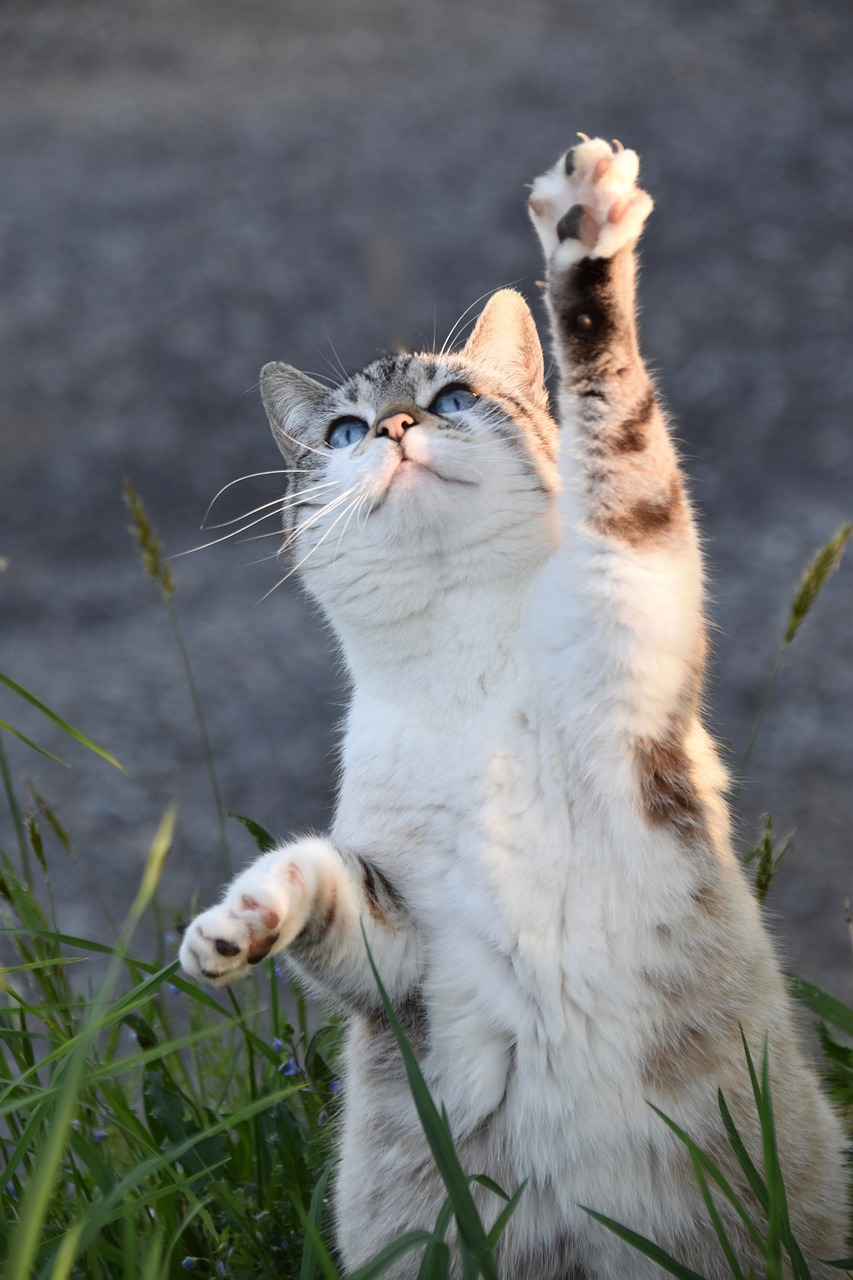
\includegraphics[width=75mm]{cat-5098930_1280.jpg}
    \caption{元画像}
    \label{img1}
  \end{center}
\end{figure}

\clearpage

\section{課題1}
コードは参考文献\cite{one}に示している通りで,画像はそれぞれ画像\ref{img2},画像\ref{img3}になっている.
\begin{figure}[htbp]
  \begin{subfigure}{0.5\textwidth}
    \centering
    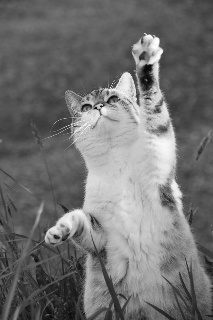
\includegraphics[width=50mm]{original.jpg}
    \caption{元画像}
    \label{img2}
  \end{subfigure}%
  \begin{subfigure}{0.5\textwidth}
    \centering
    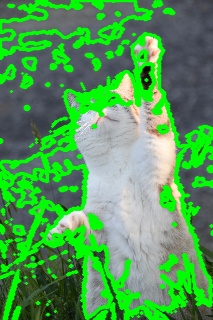
\includegraphics[width=50mm]{drawn.jpg}
    \caption{表示された画像}
    \label{img3}
  \end{subfigure}
  \caption{2つの画像の横並び}
  \label{fig:side-by-side}
\end{figure}
\subsection{面白かった点}
グレースケール化した画像\ref{img2}を見ても周りとの違いがよくわからない部分でも画像\ref{img3}を見ると輪郭として判定されていることが人間には難しい判定基準だと考える.
\clearpage
\section{課題2}
コードは参考文献\cite{two}に示している通りで,画像は画像\ref{img4}になっている.
\begin{figure}[htbp]
  \begin{center}
    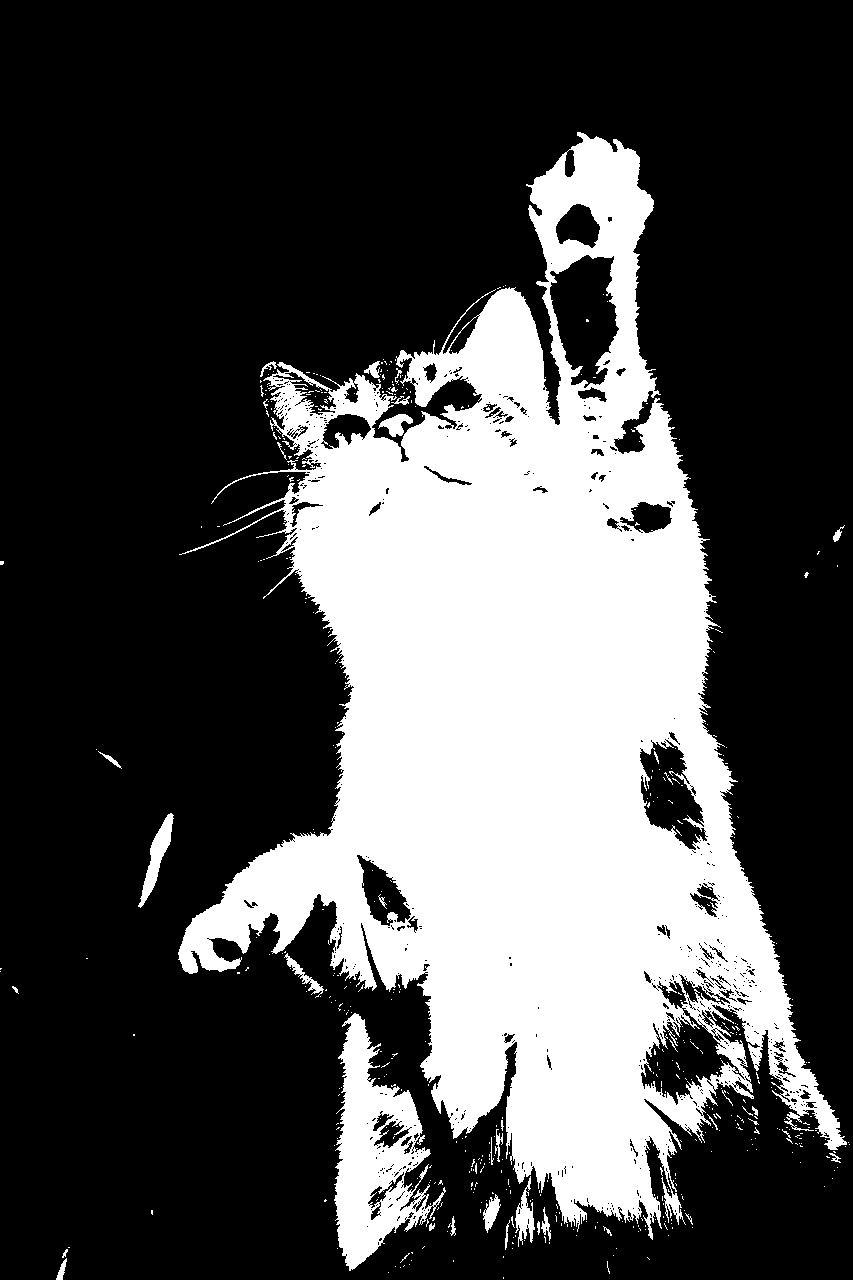
\includegraphics[width=75mm]{lena_binary.jpg}
    \caption{表示された画像}
    \label{img4}
  \end{center}
\end{figure}
\subsection{面白かった点}
元画像\ref{img1}と画像\ref{img4}比較すると二値化は色の判定が二つしかないためわかりにくい画像になっていると考える.また、輪郭の判定もこの状態では難しそうだと考える.

\section{課題3}
コードは参考文献\cite{three}に示している通りで,画像は画像\ref{img5}になっている.
\begin{figure}[htbp]
  \begin{center}
    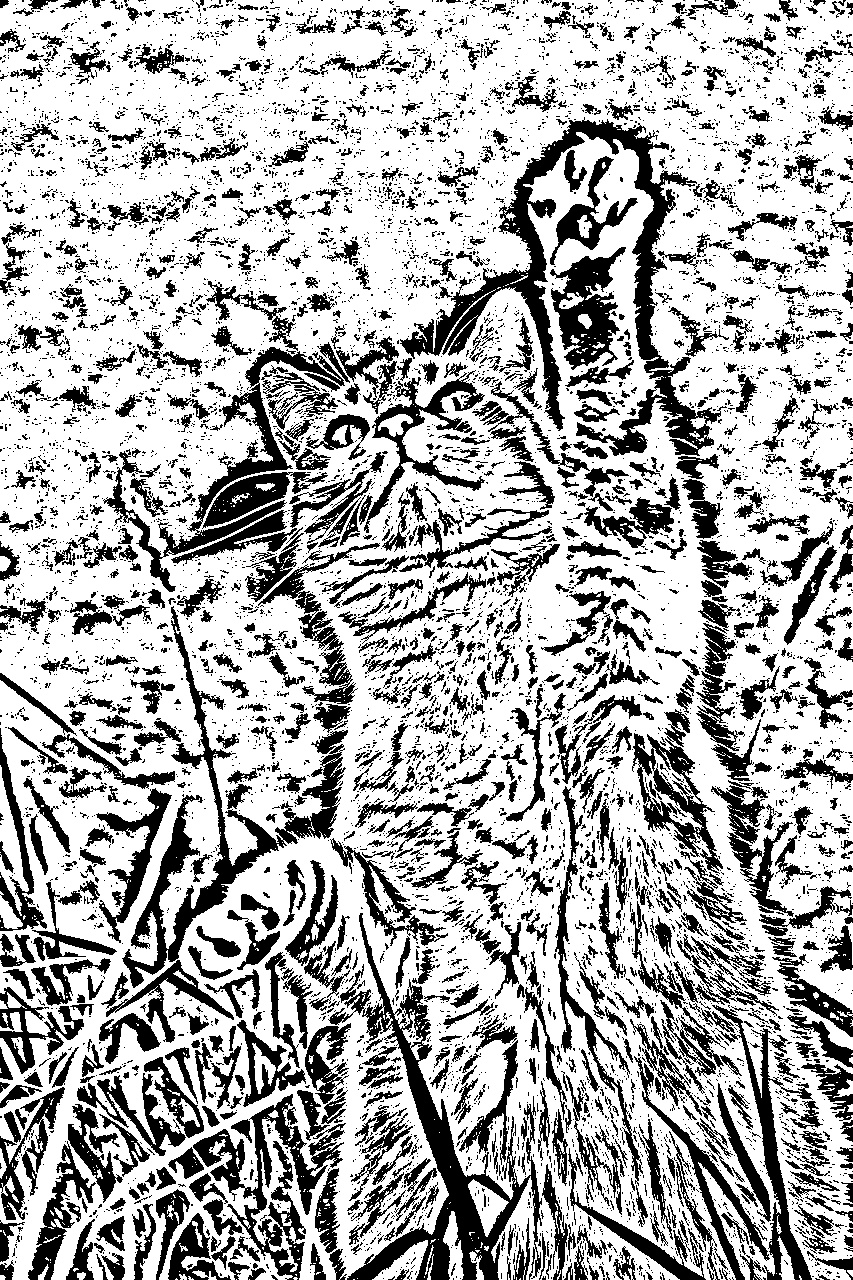
\includegraphics[width=75mm]{kirei.jpg}
    \caption{表示された画像}
    \label{img5}
  \end{center}
\end{figure}

\subsection{面白かった点}
画像\ref{img4}と画像\ref{img5}比較するとより詳細に色の判定ができるようになっていると考える.より処理をする前の画像に近くて処理工程が進んでいる感じがあった.
\clearpage
\section{課題4}
コードは参考文献\cite{four}に示している通りで,画像は画像\ref{img6}になっている.
\begin{figure}[htbp]
  \begin{center}
    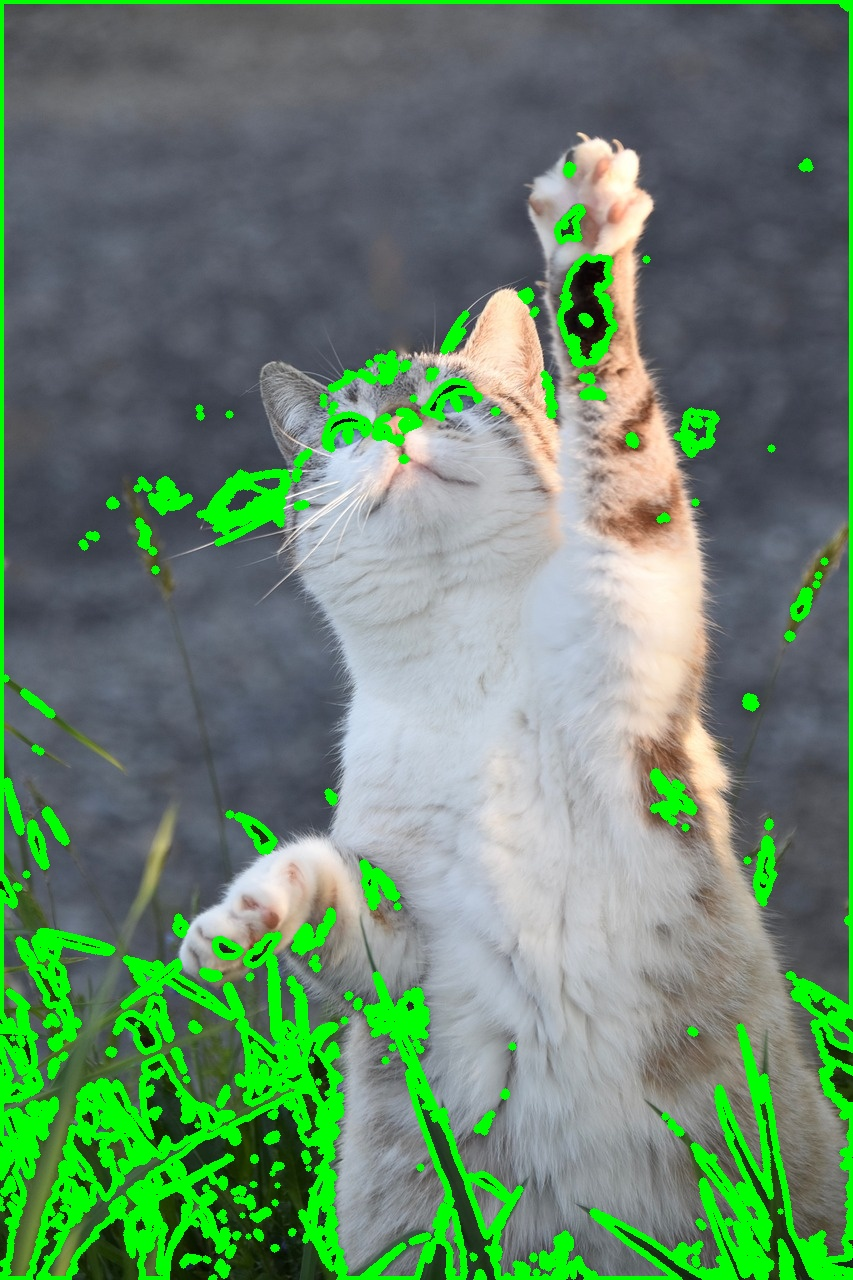
\includegraphics[width=75mm]{rinkaku.jpg}
    \caption{表示された画像}
    \label{img6}
  \end{center}
\end{figure}

\subsection{面白かった点}
画像\ref{img3}と画像\ref{img6}比較すると大まかな輪郭判定は同じだが細かい輪郭判定が違い、輪郭判定と一口に言っても判定方法が違うだけで変化すると考える.

\section{課題5}
コードは参考文献\cite{five}に示している通りで実行した.
実行したところ動いている列車のみが白で表示され視覚的にわかりやすくなっていた。
\begin{figure}[htbp]
  \begin{center}
    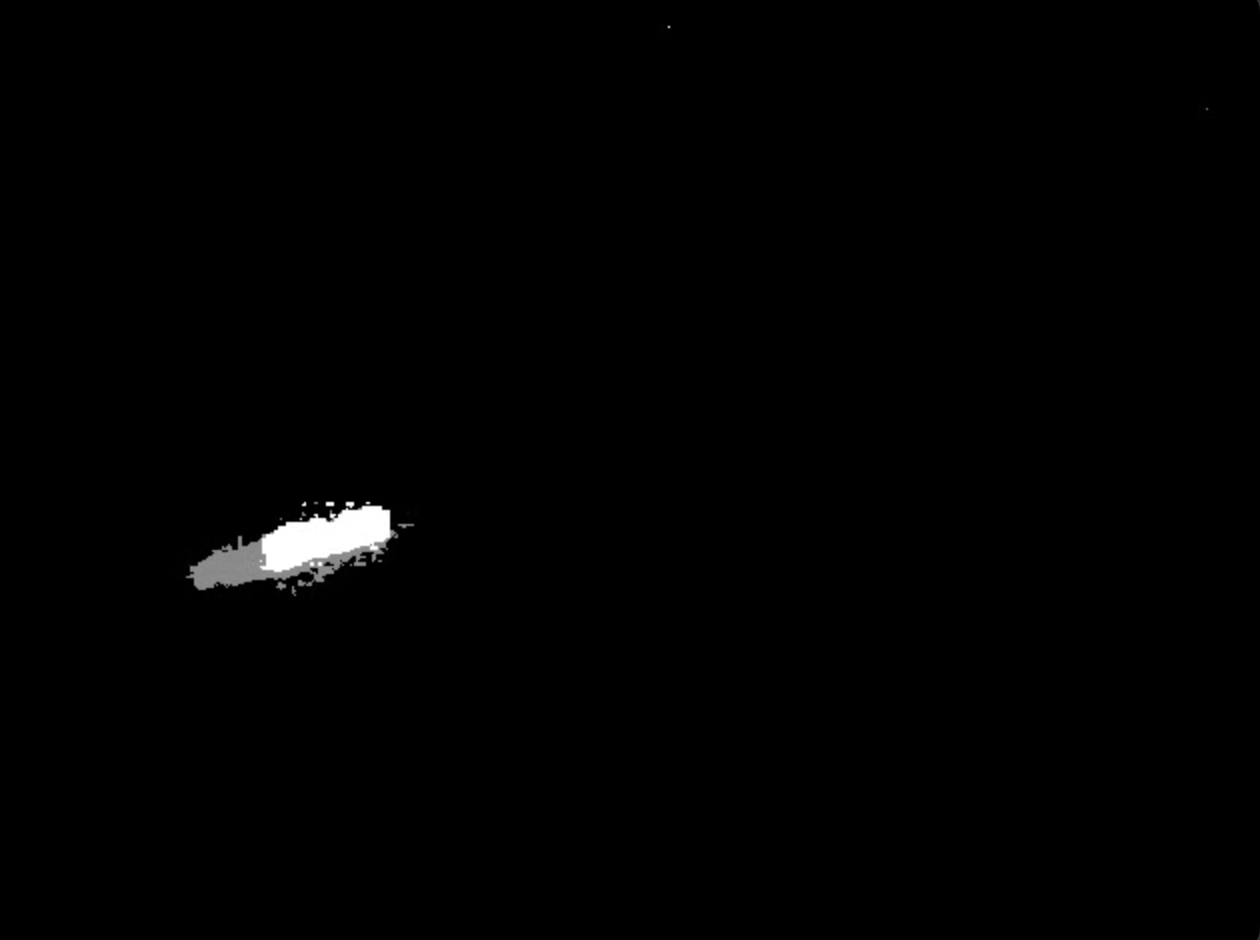
\includegraphics[width=75mm]{train.png}
    \caption{結果の一部画像}
    \label{img6}
  \end{center}
\end{figure}

\subsection{面白かった点}
画像と同様に白黒の二値化した際にはわかりにくくなると思ったが、画像と違い見やすかった.


\section{課題6}
コードは参考文献\cite{six}に示している通りで,実行したところ最初の数秒で画面中央にトラックングしその後真ん中固定でうまくトラックングできなかった.

\subsection{面白かった点}
画像と同様に白黒の二値化した際にはわかりにくくなると思ったが、画像と違い見やすかった.

\begin{thebibliography}{99}
\clearpage
\bibitem{tex} 知能情報基礎演習1講義資料「理工系のレポート作成技術」 
\bibitem{one} \href{https://www.learning-nao.com/?p=2006/}{OpenCvで画像からの物体の輪郭を検出する}
\bibitem{two} \href{https://watlab-blog.com/2019/05/25/opencv-binary/}{OpenCvでの二値化をする方法}
\bibitem{three} \href{https://watlab-blog.com/2019/05/26/opencv-adaptive-threshold/}{OpenCVの適応的閾値処理で綺麗な二値化!}
\bibitem{four} \href{https://watlab-blog.com/2020/03/19/find-contours/}{OpenCVで画像内オブジェクトの輪郭抽出をする}
\bibitem{five} \href{https://watlab-blog.com/2019/09/26/motion-detection/}{OpenCVで動体検知!動画の動いている部分を検出}
\bibitem{six} \href{https://watlab-blog.com/2020/03/21/object-tracking/}{OpenCVで動画内の物体トラッキングをする方法}
\end{thebibliography}

\end{document}
